\documentclass[10pt]{article}
\usepackage[margin=1.9cm]{geometry}
\usepackage{amsmath,amssymb}
\usepackage{booktabs}
\usepackage{tikz}
\usetikzlibrary{positioning,arrows.meta}
\usepackage[hidelinks]{hyperref}
\usepackage{microtype}

\newcommand{\T}{\tilde T}
\newcommand{\xt}{\tilde x}
\newcommand{\yt}{\tilde y}

\title{The homotopy head: a travel-time field on the double cover of SE(3)}
\author{G-NTFields, \texttt{models/graph\_homotopy}}
\date{October 2026}

\begin{document}
\maketitle

\begin{abstract}
The homotopy head is a decoder for neural time fields on SE(3). It does not decode the travel time $T(x,y)$ with a
free-form MLP. Instead, a pose encoder produces a few small per-pose quantities that enter a fixed formula built on a
free-space travel time, evaluated on the double cover $\mathbb{R}^3\times S^3$. The two lifts of the goal are the two
homotopy classes of paths in SE(3), and $T$ is the minimum over them. On 30 shape--environment cells and 30 T/L/A test
sets the head is significantly ahead of the metric NTFields on every set; on a Gibson scene it wins one of two cells.
\end{abstract}

\section{Why a double cover}
A neural time field learns $T(x,y)$, the shortest travel time between poses $x,y\in\mathrm{SE}(3)$ under a speed
$S(x)$ that falls to zero near obstacles, by fitting the Eikonal equation $\|\nabla_x T(x,y)\| = 1/S(x)$ (here with the
Lie gradient). A planner then descends $T(\cdot, y)$ towards the goal.

Rotations make this hard. $\pi_1(\mathrm{SO}(3)) = \mathbb{Z}_2$, so between two poses there are exactly two homotopy
classes of paths. $T$ is the minimum of the two class times, and where they tie (the half turn in free space, moved by
obstacles) $T$ has a ridge that a smooth network fits poorly and a gradient planner can stall on.

The double cover $\mathbb{R}^3\times S^3$ (unit quaternions, $q$ and $-q$ distinct) is simply connected. A path from $x$
to $y$ lifted from $\xt$ ends at either $\yt$ or $-\yt$: the two endpoints are the two classes. So the head learns a
field $\T$ on the cover and takes
\begin{equation}
  T(x,y) = \min\bigl(\T(\xt,\yt),\ \T(\xt,-\yt)\bigr).
\end{equation}
Each sheet $\T(\cdot,\pm\yt)$ is smooth; the only ridge of $T$ is where the sheets tie, and it is placed by the
topology rather than learned.

\section{Architecture}

\begin{figure}[h]
\centering
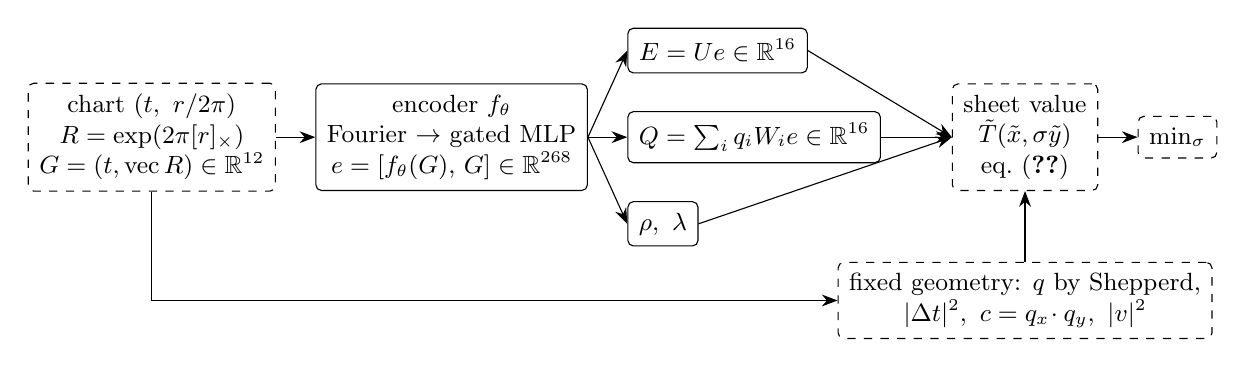
\begin{tikzpicture}[node distance=4mm and 5mm, >={Stealth[length=2mm]},
  box/.style={draw, rounded corners=2pt, align=center, inner sep=4pt, font=\small},
  fix/.style={box, dashed},
  lab/.style={font=\footnotesize, align=center}]
  \node[fix] (in) {chart $(t,\ r/2\pi)$\\$R=\exp(2\pi[r]_\times)$\\$G=(t,\mathrm{vec}\,R)\in\mathbb{R}^{12}$};
  \node[box, right=of in] (enc) {encoder $f_\theta$\\Fourier $\to$ gated MLP\\$e=[f_\theta(G),\,G]\in\mathbb{R}^{268}$};
  \node[box, right=of enc, yshift=11mm] (even) {$E=Ue\in\mathbb{R}^{16}$};
  \node[box, right=of enc] (odd) {$Q=\sum_i q_iW_ie\in\mathbb{R}^{16}$};
  \node[box, right=of enc, yshift=-11mm] (conf) {$\rho,\ \lambda$};
  \node[fix, right=9mm of odd] (sheet) {sheet value\\$\T(\xt,\sigma\yt)$\\eq.~(\ref{eq:sheet})};
  \node[fix, right=of sheet] (min) {$\min_\sigma$};
  \node[fix, below=9mm of sheet] (geo) {fixed geometry: $q$ by Shepperd,\\$|\Delta t|^2,\ c=q_x\!\cdot q_y,\ |v|^2$};
  \draw[->] (in) -- (enc);
  \draw[->] (enc.east) -- (even.west);
  \draw[->] (enc.east) -- (odd.west);
  \draw[->] (enc.east) -- (conf.west);
  \draw[->] (even.east) -- (sheet.west);
  \draw[->] (odd.east) -- (sheet.west);
  \draw[->] (conf.east) -- (sheet.west);
  \draw[->] (geo) -- (sheet);
  \draw[->] (sheet) -- (min);
  \draw[->] (in.south) |- (geo.west);
\end{tikzpicture}
\caption{Data flow. Solid boxes contain learned weights; dashed boxes are fixed computations. The pose reaches the
value twice: through the encoder, and directly through the fixed pair geometry.}
\end{figure}

\subsection{How a pose enters}
A pose is stored in the chart $(t,\,r/2\pi)$, with $t\in\mathbb{R}^3$ and $r$ the rotation vector. It is mapped,
differentiably, to $R=\exp(2\pi[r]_\times)$ and to the 12-number feature $G(x)=(t,\mathrm{vec}\,R)$. Because $G$
uses $R$, everything computed from it is the same for $q$ and $-q$. The pose is used in two separate ways:
\begin{enumerate}\setlength\itemsep{1pt}
  \item \textbf{Learned path.} $G(x)$ goes through the encoder; the per-pose heads read the result.
  \item \textbf{Fixed path.} The unit quaternion $q$ is recovered from $R$ (Shepperd's method; its sign is fixed per
        region, giving one lift $\xt$). The pair geometry is computed from $(t,q)$ with no weights at all.
\end{enumerate}

\subsection{Encoder (learned)}
The encoder is the G-Shape NTFields encoder:
\begin{align*}
  \gamma &= [\sin(2\pi G B),\ \cos(2\pi G B)]\in\mathbb{R}^{256}, && B\in\mathbb{R}^{12\times128}\ \text{fixed random
  (std 0.5 on $t$, 0.1 on $R$)},\\
  u_1 &= \sin(L_1\gamma),\quad u_2=\sin(L_2\gamma), && \text{gates,}\\
  h &\leftarrow u_1\odot\sin(Lh)+u_2\odot(1-\sin(Lh)) && \text{twice per block, then a gated residual},\\
  e(x) &= [\,L_{\mathrm{out}}h,\ G(x)\,]\in\mathbb{R}^{268}. &&
\end{align*}
There are two blocks of three $256\times256$ layers plus the output layer. The residual gate is a learned scalar,
and each weight row is softly capped at norm 1 (Lipschitz control). The raw feature $G(x)$ is appended to the output,
so the heads see the encoding and the pose itself.

\subsection{Per-pose heads (learned)}
All four heads are linear in $e(x)$:
\begin{center}\small
\begin{tabular}{llll}
\toprule
Head & Formula & Weights & Behaviour under $q\to-q$ \\
\midrule
even & $E(x)=U e$ & $U\in\mathbb{R}^{16\times268}$, no bias & unchanged \\
odd & $Q(\xt)=\sum_{i=0}^{3}q_iW_ie$ & $W\in\mathbb{R}^{64\times268}$ as $W_0..W_3\in\mathbb{R}^{16\times268}$, no bias & sign flips \\
cone scale & $\rho(x)=\mathrm{softplus}(a_\rho\!\cdot e+b_\rho)$ & $a_\rho\in\mathbb{R}^{268}$, $b_\rho$ & unchanged \\
saturation & $\lambda(x)=10^{-3}+\mathrm{softplus}(a_\lambda\!\cdot e+b_\lambda)$ & $a_\lambda\in\mathbb{R}^{268}$, $b_\lambda$ & unchanged \\
\bottomrule
\end{tabular}
\end{center}
$Q$ is linear in the quaternion, which is the only place the network sees which lift a pose is on. At initialisation
$a_\rho=a_\lambda=0$ and the biases give $\rho=0.5$, $\lambda=0.05$ everywhere.

\textbf{What is learned:} 614{,}110 parameters, of which 592{,}132 are in the encoder and 21{,}978 in the heads
($U$: 4{,}288, $W$: 17{,}152, $\rho$ and $\lambda$: 269 each). \textbf{What is fixed:} the Fourier matrix $B$, the
scales $s_t=1$ and $s_r=2\pi$ (one full turn counts as one unit, like one unit of translation), $\lambda_{\min}=10^{-3}$,
the quaternion lift and every formula in the next subsection.

\subsection{From the heads to $T$}
Take a pair with lifts $\xt,\yt$ and a sheet sign $\sigma\in\{+1,-1\}$ ($\sigma=-1$ uses the goal's other lift
$-\yt$). The value is built in five steps.
\begin{enumerate}\setlength\itemsep{2pt}
  \item \textbf{Fixed geometry.} $a=|t_x-t_y|^2$, $c=q_x\cdot q_y$, $|v|^2=1-c^2$ (with $q_x^{*}q_y=(c,v)$), and the
        rotation angle on the sheet $\psi_\sigma=2\,\mathrm{atan2}(|v|,\sigma c)\in[0,2\pi]$. On the near sheet this is
        the geodesic angle $\theta$; on the far sheet it is $2\pi-\theta$, the long way round.
  \item \textbf{Free-space cone.} $T_{\mathrm{free},\sigma}=\sqrt{a/s_t^2+\psi_\sigma^2/s_r^2}$, the exact travel time
        with unit speed.
  \item \textbf{Cone term.} Add $\bar\rho\,\bar\lambda\tanh(T_{\mathrm{free},\sigma}/\bar\lambda)$ with
        $\bar\rho=\tfrac12(\rho(x)+\rho(y))$ and $\bar\lambda$ likewise. Close to the goal
        ($T_{\mathrm{free}}\ll\bar\lambda$) the time is $(1+\bar\rho)\,T_{\mathrm{free}}$, a slower cone; beyond
        $\bar\lambda$ the term saturates to a constant offset $\bar\rho\bar\lambda$.
  \item \textbf{Even term.} Add $\|E(x)-E(y)\|^2$. It is the same on both sheets, so it is the obstacle cost that does
        not depend on the homotopy class.
  \item \textbf{Odd term.} Add $\|Q(\xt)-\sigma Q(\yt)\|^2=\|Q(\xt)\|^2+\|Q(\yt)\|^2-2\sigma\,Q(\xt)\cdot Q(\yt)$. Its learned
        values are the only ones that change between the sheets; the cone term changes only through $T_{\mathrm{free},\sigma}$.
\end{enumerate}
Together,
\begin{equation}
  \T(\xt,\sigma\yt)=T_{\mathrm{free},\sigma}+\bar\rho\,\bar\lambda\tanh\!\bigl(T_{\mathrm{free},\sigma}/\bar\lambda\bigr)
  +\|E(x)-E(y)\|^2+\|Q(\xt)-\sigma Q(\yt)\|^2,
  \qquad T(x,y)=\min_{\sigma=\pm1}\T(\xt,\sigma\yt). \label{eq:sheet}
\end{equation}
The minimum is found without gradients and only the chosen sheet is recomputed with them.

\paragraph{What each term does.}
\begin{itemize}\setlength\itemsep{1pt}
  \item \emph{The ridge.} The sheets differ through $\psi_\sigma$ (near or far way round), the cone terms, and the odd
        term, which contributes $-4\,Q(\xt)\cdot Q(\yt)$ to $\T(\xt,\yt)-\T(\xt,-\yt)$. Without obstacles $Q$ can stay small and the tie sits at the half turn; with
        obstacles $Q(\xt)\cdot Q(\yt)$ moves it, so one class can win even for rotations under a half turn.
  \item \emph{The local speed.} The squared even and odd terms have zero slope at $y=x$, so near the goal only the cone
        is felt and the Eikonal equation forces $1+\rho(y)\approx1/S_d(y)$. $\rho$ is the slowdown at a pose, and $\lambda$
        sets how far that slowdown carries.
  \item \emph{Obstacle detours.} $E$ and $Q$ add time for poses that are close in free space but far apart around
        obstacles; they add nothing when $x=y$.
\end{itemize}
By construction, for every parameter value: $T(x,x)=0$, $T(x,y)=T(y,x)$, $T\ge T_{\mathrm{free}}\ge0$, and flipping
both quaternions leaves $T$ unchanged, so $T$ is a function on $\mathrm{SE}(3)\times\mathrm{SE}(3)$.

\section{Training and planning}
\textbf{Loss.} For a training pair with endpoint speeds, take the Lie (body-frame) gradients $g_x,g_y\in\mathbb{R}^6$ of
the selected sheet with respect to each endpoint and set $N_e=S_d(e)\,\|g_e\|$, where $S_d$ is the translational
clearance speed, warped as $s^2(2-s)^2$ and clamped at $10^{-3}$. The loss is the NTFields Eikonal residual
\[
  \mathcal{L}=\beta\,\frac{1}{n}\sum_{i}\Bigl[10^{-2}\bigl(\sqrt{N_{x,i}}-1\bigr)^2+10^{-2}\bigl(\sqrt{N_{y,i}}-1\bigr)^2\Bigr]\,e^{-T_i/2},
\]
with the weight $e^{-T/2}$ emphasising short pairs. With \texttt{--lift min} each pair trains only its minimum sheet.
AdamW (learning rate $5\cdot10^{-4}$, weight decay 0.5), batches of 2000 pairs from 800k, rejected epochs rolled back,
8000 epochs.

\textbf{Planning} uses the same forward MPPI as NTFields (50 samples, horizon 5, step 0.015, temperature 50, 200
iterations). The \emph{dual} planner lifts every sample continuously and plans once towards each lifted goal $\pm\yt$,
one plan per homotopy class, keeping the plan that converges. Success means reaching the goal within 0.01 in the SE(3)
product metric with no collision on the way.

\section{Results}
Mean SE(3) success (\%) over 1000-case test sets, 3 seeds (6 on Gibson). \emph{Full} NTFields has the TD and
normal-alignment losses on; \emph{reduced} has them off. ``Ahead'' counts sets where the paired McNemar test favours the
homotopy head at $p<0.01$.

\begin{center}\small
\begin{tabular}{lrrrrr}
\toprule
Group & sets & Homotopy & Full NTF & Reduced NTF & ahead / behind \\
\midrule
New shapes, open room (env4)        & 5  & 98.0 & 90.2 & 88.0 & 5 / 0 \\
New shapes, 1 wall, 70 window (env8)& 5  & 96.7 & 89.7 & 87.3 & 5 / 0 \\
New shapes, 1 wall, 60 window (env7)& 5  & 82.8 & 73.0 & 71.6 & 5 / 0 \\
New shapes, 1 wall, 50 window (env5)& 5  & 55.6 & 51.5 & 51.3 & 5 / 0 \\
New shapes, 2 walls, 70 windows (env9)& 5 & 94.1 & 76.5 & 68.4 & 5 / 0 \\
New shapes, 2 walls, 50 windows (env6)& 5 & 33.6 & 27.7 & 26.8 & 5 / 0 \\
T / L / A, standard                 & 6  & 99.0 & 86.7 & 85.0 & 6 / 0 \\
T / L / A, long / big rotation      & 12 & 99.1 & 81.0 & 78.3 & 12 / 0 \\
T / L / A, tight / hard             & 12 & 97.0 & 66.8 & 62.9 & 12 / 0 \\
\midrule
Gibson eastville, cube              & 1  & 84.6 & 69.8 & 54.1 & 1 / 0 \\
Gibson eastville, small rectangle   & 1  & 74.0 & 88.1 & 75.9 & 0 / 1 \\
\bottomrule
\end{tabular}
\end{center}

\begin{itemize}\setlength\itemsep{1pt}
  \item The gain is in passing walls. With start and goal on the same side all models score 97--100\%. Crossing both
        walls of env9, the homotopy head scores 87.2\% against 49.0\% (full NTFields).
  \item Narrow 50-unit windows (env5, env6) defeat both methods: crossing one wall succeeds in 11--15\% of cases for the
        homotopy head and about 4--5\% for NTFields.
  \item The one loss is the small rectangle in eastville, where the homotopy head collides in 24\% of cases against
        10\% for the full NTFields.
\end{itemize}

\end{document}
